\section{事故096-1-A}

\label{sec:DOC-incident-096-1-a}

\ii{“那么收容成功了?”}

\ii{“是的,博士。”}

\ii{“给我看看安保录像。”}

\begin{scpbox}

\bb{<记录开始>}\\
\\
\ii{某个塞了大概一打研究员的实验室中间放着一个巨大的钢制立方体。摄像机视野中有一个控制室,正显示着立方体内部各种传感器的示数。}

{[}快进一分钟三十二秒]

\ii{控制室的操作员身体前倾,注意到传感器的示数不对头。约五秒后,收容立方体的一面钢墙上出现了一个相当大的凸起。凸起越变越大,最终裂开了。可看到SCP-096正掰开钢板,发疯似的试图逃跑。收容突破警报响起,同时应急钢板罩到立方体上。}

{[}安保录像带上SCP-096的脸依照收容方案做了模糊处理]

\ii{两个安保小组在SCP-096脱离收容室时进入了房间。实弹和镇静剂飞镖均未造成可见的效果。大约90\%的研究员和安保人员直接看到了SCP-096的脸,此时宣布执行代号L方案。研究室和周边区域被封锁并充入██-级神经毒气。}

\ii{约两分钟后SCP-096逃出██号研究站点,以██km\slash h的速度穿过外面的沙漠,冲向████。}\\
\bb{<记录结束>}

\end{scpbox}

\ii{“Echo Romeo-Actual被派来处理当前的收容突破。当我们意识到我们正在对付一次多么严重的突破的时候,我们完全无法应付。真好笑,世界上最好最聪明的头脑们居然会这么措手不及。”}

\ii{“所以你是说这是你的错?”}

\ii{“绝对不是。这是对SCP-096行为的一个新发现。我们以前没办法知道,幸好这没变成一次XK事件。”}

\begin{scpbox}

\bb{<记录开始>}

\bb{ER-A 5头盔摄像机的录像}

{[}从一架UH-60“黑鹰”直升机内部拍摄的画面显示SCP-096在沙漠上高速移动。]\\
\\
ER-A 1:这里是Echo Romeo-Actual。我们看见目标了!-无法听清-……{[}数据删除]节(译注:“节”,速度单位),还在加速!

\ii{ER-A 1在听无线电播送的命令(听得出是来自Dan博士)。可看到SCP-096正在缓慢加速。}

\ii{ER-A 1离开镜头视野。ER-A 3出现,手持一把改造过的XM500反器材步枪。两发子弹出膛:第一发打偏了,第二发击中了SCP-096的小腿。SCP-096打了个趔趄,但又恢复了。速度无明显变化。}

ER-A 1:-无法听清- ……复,对目标无效!

\ii{ER-A 1再次向ER-A 3示意。ER-A 3又开了三枪:头两枪射偏,第三枪命中SCP-096头部。SCP-096倒地,滑行,翻滚了若干圈,速度稍有降低。SCP-096站起,继续前行,势头不减。}

\ii{镜头上拉,拍摄到八架V-22“鱼鹰”倾转旋翼机(隶属于机动特遣队Tau-1)从上空飞过,掠过直升机,飞往SCP-096离开的方向。摄像机关闭。}

\bb{<记录结束>}

\end{scpbox}

\begin{scpbox}

\bb{<记录开始>}

\bb{采访视频记录096-1-A}

{[}Oleksei博士看上去镇定自若,缓慢而谨慎地回答所有问题。]

\bb{采访者:}收容突破的时候你的准确位置在哪里?

\bb{Oleksei博士:}在休息,正在取一杯咖啡。我没被关在收容区域里只是运气好。

\bb{采访者:}描述你在收容刚被突破时的行动。

\bb{Oleksei博士:}我派Echo Romeo-Actual去追SCP-096并向Dan博士通报了情况。之后我们开始为SCP-096-1定位。一确定SCP-096的大致去向,我就派出了机动特遣队Tau-1去SCP-096路径上的人口中心提前疏散平民。一切按照收容方案进行。

\bb{<记录结束>}

\end{scpbox}

\begin{scpbox}

\bb{<记录开始>}

\bb{采访视频记录096-1-B}

{[}Daniel █████博士耐心地坐着。他面前的桌上放着一套看起来是改造过的夜视护目镜的东西。]

\bb{采访者:}为了作记录,请问SCP-096突破收容的时候你的准确位置在哪里?

\bb{Dan博士:}在{[}数据删除]山脉,想找到更多关于SCP-096来历的信息。这是一次短期的研究考察,所以我让Oleksei博士管理收容。他足以胜任,虽然有点儿……热切,而且过去他也证明过自己。这些都是有各种文件证据的,所以请不要认为——

\bb{采访者:}作个记录而已,博士。那么,你明知道SCP-096在被激怒的时候不受任何已知形式的伤害影响,为什么还命令应急反应小队进行狙击呢?

\bb{Dan博士:}为什么不?如果有可能让SCP-096慢下来,给特遣队Tau-1争取更多时间,我们就必须试试。这对ER-A没有威胁,而且当时直升机有追不上的危险。说实话,ER-A几乎没有其它让局面好转或者恶化的办法。

\bb{采访者:}我明白了。那你能解释这个吗?

{[}采访者指了指桌上的护目镜]

\bb{Dan博士:}好的。这是Project SCRAMBLE,我和Oleksei博士专门针对SCP-096设计的护目镜,发给了ER-A和特遣队Tau-1。它有一个不停分析视野来寻找SCP-096面部特征的微处理器。内部的面部识别软件将立即识别出它们,在光线到达人眼之前把那部分图像抹成无法辨认的一团。这真的很精巧。

\bb{采访者:}而且昂贵。

\bb{Dan博士:}非常贵。所以它没起作用真是太可惜了。

\bb{<记录结束>}

\end{scpbox}

\begin{scpbox}

\bb{<记录开始>}

\bb{机动特遣队(MTF)Tau-1与经改造的EG-3“哨兵”预警机(呼号为“老大哥”)之间通信的文字记录\footnote{译注:预警机型号在网络资料中均为“E-3”,此处疑为笔误}}

\bb{MTF-T-1:}鱼鹰在天上,以{[}数据删除]向{[}数据删除]移动。等待方向指示。

\bb{老大哥:}电子设备启动,到达巡航高度。正在向所有摄像系统上传SCRAMBLE程序……摄像头启动。老大哥正在观测。

\bb{MTF-T-1:}目标现在向哪个方向去了?

\bb{老大哥:}目标正向西行进……处在……操。好吧,他在I-40上。我想他刚撞翻一辆卡车。唔,方向是……{[}数据删除]偏{[}数据删除]度。这个方向上的下一个城镇是……{[}数据删除]。我觉得还有几百公里。操……MTF,我们建议Echo Romeo开始疏散I-40上的人员。我不知道目标已经毁掉多少辆车了。

\bb{MTF-T-1:}等一下。不行,老大哥。ER-A报告说目标比他们的直升机快。他们没办法赶到前面。

\bb{老大哥:}那就让他们去把另一条车道上的司机拦下来……我不知道有多少人看过了这家伙的脸。

\bb{<记录结束>}

\end{scpbox}

\ii{“Tau-1的前三组人成功地平安集合了头三个城镇的居民。SCP-096依次穿过这几个地方而没有停下,证明SCP-096-1不在里边。然而,MTF-Tau的一份视频记录显示了{[}数据删除]城里被找到的SCP-096-1,还有接下来的事故。”}

\ii{“放吧。”}

\begin{scpbox}

\bb{<记录开始>}

\bb{{[}数据删除]城中MTF-Tau-1第四组的头盔摄像机的录像}

\ii{大部分居民被集中到广场上,都蒙上了眼睛。直升机扫视着城镇。从直升机上和地面人员的扬声器里传出模糊的命令。}

\bb{MTF-T-1(通过队内通讯频道和扬声器):}标正在进入临近地带!所有单位启动SCRAMBLE装置,开始执行人群管制程序!所有平民不许离开原地或者摘除眼罩!移动或触摸眼罩的人会被射击!重复,所有平民——{[}从摄像机视野外传来的一声响亮的尖叫盖过了命令]

\ii{约两公里外,可看到SCP-096正翻过山顶。它试着在山坡上减速,却绊倒了,高速滚下山丘,撞穿数幢房屋后又几乎立刻站稳。}

\bb{扬声器中传出的身份不明的声音:}{[}无法听清]……平民不许移动!开枪了!重……{[}无法听清]

\ii{听到几声枪响,都不是对着SCP-096开的枪。SCP-096停了一秒钟,冲进人群,扔开不少人,被踩踏的更多。人群开始四散,枪声再次响起,扬声器的声音在SCP-096的叫声之下无法辨认。SCP-096找到了SCP-096-1,一名中年男子。摄像机拍到SCP-096抓住了他,之后摄像机被一名逃跑的居民撞到,从头盔上落下。}

\bb{<记录结束>}

\end{scpbox}

\begin{scpbox}

\bb{<记录开始>}

\bb{采访视频记录096-1-C}

**Jack Wilford少校(MTF Tau-1现任指挥官):当时我和我的队伍在搜查SCP-096-1的房子。那可怜虫是个半职业的登山运动员,爬过█████████。显然他照了一张风景照,碰巧看到了背景里的SCP-096。

{[}Wilford伸出四根手指以示强调]

\bb{Wilford:}四个像素。麻痹的四个像素。我怀疑他都不知道看到了什么。他可能就是看了一下照片,注意到有一小块雪没颜色,然后继续过这一天。

\bb{采访者:}你怎么找到的?

\bb{Wilford:}我们的SCRAMBLE装置马上就把它认出来了。中尉拿到了照片,在我有机会看到它之前就把它带上直升机了。在那之前那个该死的怪物已经把老大哥弄了下来,还撕开了{[}前任]少校的“斯特瑞克”\footnote{译注:美军使用的一种装甲车}。太乱了。

\bb{采访者:}所以SCRAMBLE装置没起效?

\bb{Wilford:}没起效?他娘的SCRAMBLE就是一堆屎,害死了整支特遣队。你知不知道加上我只有三个人活下来?都是因为有些弱智学究想的什么“最先进的SCP-096敌意反应对策”。那些混账白痴明明只需要往目标头上套个袋子就完事了,但是不行,我们必须得用最他妈先进的SCRAMBLE。

\bb{<记录结束>}

\end{scpbox}

\begin{figure}[H]
    \centering
    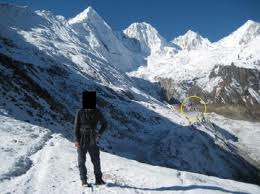
\includegraphics[width=0.5\linewidth]{images/incident-096-1-a.jpg}
    \caption*{MTF-Tau取回的照片。SCP-096在黄圈中,已遮挡。}
\end{figure}

\begin{scpbox}

\bb{<记录开始>}

\bb{Dan博士:}那个杂种叫我什么?

{[}Dan博士往桌子后一挪,开始站起来]

\bb{Dan博士:}我要让那个狗娘养的瞧瞧学究是干什么的,我要砸烂他的——{[}被采访者开始破口大骂。]

{[}两名守卫进入房间,将Dan博士按回座位]

\bb{采访者:}需要镇静剂吗,博士?

{[}Dan博士吸了一口气,整理好外套]

\bb{Dan博士:}不,不用。我道歉。{[}叹气]SCRAMBLE真的是一个非常巧妙的主意。但是它失败了,因为我们并没有完全理解SCP-096是如何运作的。你看,SCRAMBLE里的芯片识别出SCP-096的面部特征并开始打乱它们的时候,有一个瞬间,没受干扰的光线到达了视网膜。计算机很快,但没有光那么快。所以,大脑在一瞬间内接收到了SCP-096的脸部图像。那甚至都没被意识到,但显然已经足够激发SCP-096的敌意反应了。

\bb{采访者:}所以,加上这份照片的报告……

\bb{Dan博士:}这是整个事故里最令人不安的部分。你知道上一个SCP-096-1是什么时候爬那次山的吗?199█年。那张照片挂了██年他才看到SCP-096。既然大脑不需要意识到看到了SCP-096的脸就能触发反应,那世界上名副其实的“任何地方”都可能藏着定时炸弹。外面有多少张照片里有还没被注意到,等着一双细心的眼睛的SCP-096?还是那句话,我希望那家伙被处决。现在。

\bb{<记录结束>}

\end{scpbox}

\ii{“只是一个小问题,博士。嗯,你当时到底打算干什么?我们招募Jack Wilford少校的时候他可是最好的SBS队员\footnote{译注:英国皇家海军特别舟艇队}。”}

\ii{“我以前也是个强侦连(译注:美国海军陆战队强侦连)医疗兵,曾经被部署在高加索,长官。海军陆战队比SBS强。”}

\ii{“不,他们不行。”}

\ii{“你们两个够了。继续。”}

\begin{scpbox}

\bb{<记录开始>}\\
\bb{采访视频记录096-1-D}

\bb{一级军士长████(ER-A的舱门机枪手):}我把袋子套在了它头上。

\bb{采访者:}是的,你已经告诉过我了。你能告诉我当时究竟发生了什么吗?

\bb{████:}它……它完事了,它那些……它坐在那儿,公路上。刚刚毁掉一辆面包车。{[}被采访者沉默了。]

\bb{采访者:}然后呢?

\bb{████:}我……Wes降落了直升机;我出去给它套袋子。我把袋子套在它头上。它冷静了下来,然后他们把它带走了。

\bb{采访者:}所以面包车里的遇难者是最后看到SCP-096的脸的人?

{[}被采访者沉默了]

\bb{采访者:}████?

{[}被采访者在采访余下的时间里一直沉默。之后他被发现在自己的宿舍用一根凑合的绳子上吊自杀了,拳头里攥着一个半变形的奶嘴。]

\bb{<记录结束>}

\end{scpbox}

\begin{scpbox}

\bb{<记录开始>}\\
\\
\bb{视频记录096-1-D,从新闻电视台“CNN”没收的录像带}

{[}画面上越过外景记者的肩膀看去,第一反应员\footnote{译注:first responder,事故发生后首先抵达现场展开救援工作的人员}围着一架坠毁飞机的残骸。]

\bb{记者:}这架似乎本来用于军事的飞机外表上没有表明其属于美國軍方的标志。第一反应员正在寻找黑匣子记录,同时警方认为这架飞机是由于驾驶舱和机身都受到严重破坏而坠毁的。

{[}记者指向飞机一侧的一个大洞,几个消防员正向里爬。]

\bb{记者:}医务人员只找到三具尸体,这对于一架看上去大约需要二十名机组成员的飞机来说很奇怪。警方暗示——

{[}记者被打断了,因为三架“超级种马”直升机出现在上空,其中两架着陆,里面走出属于MTF-Epsilon的部队。]

\bb{MTF-E-1:}关掉摄像机。他妈的关掉——

\bb{<记录结束>}

\end{scpbox}

\begin{scpbox}

\bb{<记录开始>}

\bb{Oleksei博士:}那么我们谈完了吗?

\bb{采访者:}最后一个问题,博士。或者更像是一个说明。我们觉得很有意思:██号研究站点里没有休息室。也没有咖啡。

{[}被采访者保持沉默。]

\bb{采访者:}我们觉得你最好说点什么。

{[}采访视频记录096-1-A的剩余部分被编辑]

\bb{<记录结束>}

\end{scpbox}

\ii{“我不明白这跟我有什么关系。”}

\ii{“没必要装傻,博士。他全都说了。”}

\ii{“……好吧,我想再装作什么样子都没用了,是吗?”}

\begin{scpbox}

\bb{音频记录,O5听证会}

\bb{O5-1:}根据对你的证词、可用的录像以及已故的Oleksei博士的供词的重新审查,O5一致认为你应被处决,因为你在SCP-096的严重突破中的角色——

\bb{Dan博士:}我以为你明白“顾全大局”的含义。

\bb{O5-1:}不要考验我的耐心,博士。鉴于此次事故的影响范围和潜在可能性,O5通过了你处决SCP-096的请求。考虑到缺乏了解SCP-096的人员,处决交给你负责,在重兵守卫和我的亲自监督下执行。对你的处决将安排在之后的某天。

\bb{<记录结束>}

\end{scpbox}

\ii{“那太可怕了,博士。你怎么能故意——”}

\ii{“这样管用。那种事总有一天会发生在大型的人口中心,它的脸也迟早会传遍全世界的新闻。我可以杀掉096,但在这过程中,我已经杀掉了我自己。”}
